% Basic stuff
\documentclass[a4paper,10pt]{article}
\usepackage[nswissgerman]{babel}

% 3 column landscape layout with fewer margins
\usepackage[landscape, left=0.75cm, top=0.75cm, right=0.75cm, bottom=1.25cm, footskip=10pt]{geometry}
\usepackage{flowfram}
\ffvadjustfalse
\setlength{\columnsep}{0.75cm}
\Ncolumn{3}

% define nice looking boxes
\usepackage[many]{tcolorbox}

% a base set, that is then customised
\tcbset {
    base/.style={
	boxrule=0mm,
	leftrule=1mm,
	left=1.75mm,
	arc=0mm, 
	fonttitle=\bfseries, 
	colbacktitle=black!10!white, 
	coltitle=black, 
	toptitle=0.75mm, 
	bottomtitle=0.25mm,
	title={#1}
    }
}

\definecolor{brandblue}{rgb}{0.34, 0.7, 1}
\newtcolorbox{mainbox}[1]{
	colframe=brandblue, 
	base={#1}
}

\newtcolorbox{subbox}[1]{
	colframe=black!20!white,
	base={#1}
}
\definecolor{badred}{rgb}{0.96, 0.26, 0.21}
\definecolor{goodgreen}{rgb}{0.22, 0.56, 0.24}

% Mathematical typesetting & symbols
\usepackage{amsthm, mathtools, amssymb} 
\usepackage{marvosym, wasysym}
\usepackage{xfrac}
\usepackage{siunitx}
\allowdisplaybreaks

% Tables
\usepackage{tabularx, multirow}
\usepackage{makecell}
\usepackage{booktabs}
\renewcommand*{\arraystretch}{2}

% Make enumerations more compact
\usepackage{enumitem}
\setitemize{itemsep=0.5pt, leftmargin=0.5cm}
\setenumerate{itemsep=0.75pt, leftmargin=0.5cm}
\let\svitem\item
\newenvironment{citemize}[1][\relax]{\renewcommand\item[1][black]{\color{##1}\svitem}
  \ifx\relax#1\itemize\else\itemize[#1]\fi}{\enditemize}

% To include sketches & PDFs
\usepackage{graphicx}
\usepackage{wrapfig}

% For hyperlinks
\usepackage{hyperref}
\hypersetup{
	colorlinks=true
}

% No newline after subsubsections
\usepackage[compact]{titlesec}
\titleformat{\subsubsection}[runin]{\bfseries}{}{0pt}{}[]

% Metadata
\title{Cheatsheet\\ Visual Computing}
\author{Julian Steinmann}
\date{\vspace{-10pt}Winter 2023}

\newcommand*\good{\item[goodgreen]}
\newcommand*\bad{\item[badred]}

\begin{document}

\maketitle

\renewcommand{\abstractname}{License}
\begin{abstract}
	This document is licensed under CC BY-SA 4.0. It may be distributed or modified, as long as the author and the license remain intact.

	\begin{center}
	    The \LaTeX source code is available at \\ \href{https://github.com/XYQuadrat/eth-cheatsheets}{\color{brandblue}github.com/XYQuadrat/eth-cheatsheets}.
	\end{center}
\end{abstract}

\section{Computer Vision}
\subsection{The digital image}
An image is a representation of a continuous function. A pixel is a discrete sample of that function.

Digital images have many challenges: transmission interference, compression artifacts, spilling, scratches, sensor noise, bad contrast / resolution, motion blur.

\begin{subbox}{Charge Coupled Device (CCD)}
    An array of photosites capture photons and hold a charge proportional to the light intensity.
    We measure the charge with an analog-digital converter (ADC) line by line.
    \begin{citemize}
        \bad Blooming: finite bucket capacity, oversaturation causes bright vertical line
        \bad Bleeding/smearing: happens only with electronic shutters, worse for shorter shutter times
        \bad Dark current: thermally generated charges yield noise despite darkness, worsens with age
    \end{citemize}
\end{subbox}

\begin{subbox}{CMOS}
    Every sensor has its own amplifier, otherwise similar to CCD.
    Is cheaper, lower power, has random pixel access and no blooming but is less sensitive and has more noise.
    Rolling shutter can be an issue if we read out line by line.
\end{subbox}

\begin{mainbox}{Nyquist-Shannon sampling theorem}
    The sample rate must be at least twice as big as the largest frequency of the sampled signal to avoid aliasing.
\end{mainbox}

\noindent Bilinear interpolation: \(f(x,y) = (1-a)(1-b) \cdot f(i,j) + a(1-b) \cdot f(i+1,j) + ab \cdot f(i+1, j+1) + (1-a)b \cdot f(i,j+1)\) \\
Geometric resolution: \# of pixels per area \\
Radiometric resolution: \# of bits per pixel 

\subsection{Image Segmentation}
\subsubsection{Complete partition} 
Finite set of non-overlapping regions \( R_1, \dots, R_n \) s.t. \( I = \bigcup_{i=1}^N R_i \) (covers the whole image). 

\subsubsection{Thresholding} 
label pixel in or out by comparing with a threshold T

\subsubsection{Chromakeying}
use special background color if segmentation is desired 

\subsubsection{Mahalanobis distance} 
more sophisticated segmentation formula (accounts for variance): \( \sqrt{(x - \mu)^\top \Sigma^{-1}(x - \mu)} > T \), \( T \) is threshold. \( \Sigma  \) is the covariance matrix\\ \( \Sigma_{ij} = \mathbb{E}\left[(X_i - \mu_i)(X_j - \mu_j) \right] \), estimate from \( n \) data points: \( \frac{1}{n-1} \sum_{i=1}^{n} (x_i - \bar{x})(x_i - \bar{x})^\top \)

\subsubsection{ROC curve} 
Describes performance of binary classifier. X-axis is \( \sfrac{\text{FP}}{\text{FP}+\text{TN}} \), the y-axis is \( \sfrac{\text{FP}}{\text{FP} + \text{TN}} \). We can choose operating point with gradient \( \beta = \frac{N}{P} \frac{V_{TN} + C_{FP}}{V_{TP} + C_{FN}} \) with \( V \) being value and \( C \) being cost.

\subsubsection{Pixel neighbourhoods}
To improve segmentation: consider local pixels. Either 4-neighb. (horizont./vert. adjacent) or 8-neighb. (+ diagonals)

\subsubsection{Region growing}
Start from seed point, add neighbouring pixels with shared property (e.g. Mahalanobis dist.), then iterate

\subsubsection{Background subtraction}
Simple: \( I_\alpha = \left| I - I_{bg} \right| < T \), better: \( I_\alpha = \sqrt{(I-I_{bg})^\top \Sigma^{-1} (I-I_{bg})}  \)

\subsubsection{Morphological operators} 
Logical transformations based on comparisons: \textit{erode} (delete FG pixels with 8-conn. BG pixels), \textit{dilate} (add FG pixel to every 8-connected FG pixel), combination useful for smoothing / removing noise

\subsection{Image Filtering}
\begin{itemize}
    \item \textbf{separable} - if we can write a kernel as a product of two (usually simpler) filters. Gaussian is separable
    \item \textbf{shift invariant} - kernel does the same for all pixels
    \item \textbf{filter at edges} - clip to black, wrap around, copy edge, reflect across edge, vary filter near edge
\end{itemize}
\begin{mainbox}{Correlation}
    Compare how similar \( I'(x,y) = \sum_{(i,j) \in N(x,y)} K(i,j) \cdot I(x+i,y+j) \) patch is to correlation mask (template matching).
\end{mainbox}

\begin{mainbox}{Convolution}
    \( I'(x,y) = \sum_{(i,j) \in N(x,y)} K(i,j) \cdot I(x-i, y-j) \)\\
    For the continous case: \( g(x) = f(x) * k(x) = \int_\mathbb{R} f(a) k(x-a) \mathop{da}  \)\\
    Convolution is linear, associative, shift-invariant and commutative if the dimensions are identical.
\end{mainbox}

\subsection{Kernel examples}
\bgroup
\setlength{\tabcolsep}{0.2em}
\begin{tabularx}{\linewidth}{lllX}
    Low-pass & \( \frac{1}{9} \left[\begin{smallmatrix} 1 & 1 & 1 \\ 1 & 1 & 1 \\ 1 & 1 & 1 \end{smallmatrix}\right]  \) & 
    High-pass & \( \left[\begin{smallmatrix} -1 & -1 & -1 \\ -1 & 8 & -1 \\ -1 & -1 & -1 \end{smallmatrix}\right]  \) \\
    Laplacian & \( \left[\begin{smallmatrix} 0 & 1 & 0 \\ 1 & -4 & 1 \\ 0 & 1 & 0 \end{smallmatrix}\right]  \) &
    Prewitt (y-dir) & \( \left[\begin{smallmatrix} -1 & -1 & -1 \\ 0 & 0 & 0 \\ 1 & 1 & 1 \end{smallmatrix}\right]  \) \\
    Sobel (y-dir) & \( \left[\begin{smallmatrix} -1 & -2 & -1 \\ 0 & 0 & 0 \\ 1 & 2 & 1 \end{smallmatrix}\right]  \) &
    Band-pass & high \(*\) low \\
    Diff. (x) & \( \left[\begin{smallmatrix} -1 & 1 \end{smallmatrix}\right] \) &
    Roberts (y-dir) & \( \left[\begin{smallmatrix} 0 & 1 \\ -1 & 0 \end{smallmatrix}\right] \) \\
    Diff. (y) & \( \left[\begin{smallmatrix} -1 \\ 1 \end{smallmatrix}\right] \) &
    Gaussian (\( G_\sigma \))  & \( \frac{1}{2\pi \sigma^2} e^{-\frac{x^2+y^2}{2\sigma^2}} \) \\
\end{tabularx}
\egroup
The Gaussian kernel is rot. symmetric, single lobe, FT is again Gaussian, separable.

\subsection{Edge detection}
An edge is a sudden change in brightness. The location is the max. of the first derivative.
\subsubsection{Laplacian zero-crossings} Find 0's in \( I'' \) by applying Laplacian kernel to \( I \). This yields very noisy but thin and uninterrupted edges. Very sensitive, so blur first (Laplacian of Gaussian) or suppress edges with low gradient magnitude
\subsubsection{Canny edge detector} Has thin interrupted edges that are extended more completely than with simple thresholding
    \begin{enumerate}
	\item Smooth image with Gaussian
	\item Compute grad. mag. and orientation (Sobel, Prewitt, ...)
	\item Non-maxima suppresion: quantize edge normal to one of four dirs, if mag. \( <\) either neighbour then suppress, else keep
	\item Double thresholding: \( T_{high}, T_{low} \), keep if \( \ge T_{high} \) or \( \ge T_{low} \) and 8-connected through \( \ge T_{low} \) to a \( \ge T_{high} \) pixel
    \end{enumerate}
\subsubsection{Hough transform} Fits straight lines to edge pixels (\( y = mx + c \))
    \begin{enumerate}
	\item Subdivide \( (m, c) \)-space into discrete bins with value 
	\item Draw a line in \( (m,c) \)-space for each edge pixel and increment bins by 1 along line
	\item Detect peaks, e.g. by thresholding after non-maximum suppresion
    \end{enumerate}
    Infinite slopes are a problem, so reparametrize line with \( (\Theta , p): \; x \cdot \sin (\Theta )- y \cdot \cos (\Theta ) + p = 0 \). For detecting circles with known radius use \( (x-a)^2+(y-b)^2 = r^2 \)
\subsubsection{Harris corner detection} Scan picture with a given window size and compute the second moment matrix \( M = \left[\begin{smallmatrix}\sum I_x(x,y)^2 & \sum I_x(x,y)\cdot I_y(x,y) \\ \sum I_x(x,y)\cdot I_y(x,y) & \sum I_y(x,y)^2 \end{smallmatrix}\right] \). Then compute \( C(x,y) = \det(M) - k\cdot (\text{trace}(M))^2 = \lambda_1 \cdot \lambda_2 - k(\lambda_1 + \lambda_2)^2 \) and mark as corner if \( c(x,y) > T \). Do non-maximum suppression to avoid duplicate detections and for better localization, add gaussian weighting to all terms in \( M \): \( G(x-x_0, y-y_0, \sigma) \). Invariant to shift, rotation and brightness offset but not scaling
\subsubsection{Scale Invariant Feature Transform (SIFT)} Useful to find corresponding feature points in two images. Approach: Look for strong responses of Difference of Gaussian (DoG) over scale space and position, consider local maxima in both spaces to find blobs. Compute histogram of gradient directions (ignoring gradient mag. because of lighting etc.) at selected scale and position and correct rotation by choosing principal direction. Now both pictures are at the same scale \& orientation, so we can compare gradient histograms to find matching points. \[
	\text{DoG}(x,y) = \frac{1}{k} e^{\frac{x^2+y^2}{(k\sigma)^2}} - e^{-\frac{x^2+y^2}{\sigma ^2}}, \quad \text{e.g. } k=\sqrt{2} 
\] 

\subsection{Fourier Transform}

\begin{mainbox}{The Fourier Transform}	
    The Fourier Transform (FT) represents a signal \( f \) in terms of amplitudes and phases of its constituent sinusoids.\\
    1D: \[
	F(u) = \int_\mathbb{R} f(x) \cdot e^{-i2\pi ux} \mathop{dx}
    .\] 
    2D: \[
	F(u,v) = \iint_{\mathbb{R}^2} f(x,y) \cdot e^{-i2\pi(ux + vy)} \mathop{dx} \mathop{dy}
    .\] 
    \( e^{-i2\pi (ux+vy)} = \cos (2\pi (ux+vy)) + i \cdot \sin(2\pi (ux + vy)) \)
\end{mainbox}

\subsubsection{Properties of the FT}
\begin{center}
    {\renewcommand{\arraystretch}{1.2}
    \begin{tabularx}{\linewidth}{Xll}
	\toprule
	Property & \( f(x) \) & \( F(u) \) \\
	\midrule
	Linearity & \( af_{1}(x) + bf_{2}(x) \) & \( aF_{1}(u) + bF_{2}(u) \) \\
	Duality & \( F(x) \) & \( f(-u) \) \\
	Convolution & \( (f*g)(x) \) & \( F(u) \cdot G(u) \) \\
	Product & \( f(x) \cdot g(x) \) & \( (F*G)(u) \) \\
	Timeshift & \( f(x -x_{0}) \) & \( e^{-2\pi i ux_{0}} \cdot F(u) \) \\
	Freq. shift & \( e^{2\pi i u_{0}x} f(x) \) & \( F(u - u_{0}) \) \\
	Differentiation & \( \sfrac{\mathop{dn}}{\mathop{dx^n}} f(x) \) & \( (i_{2}\pi u)^n F(u) \) \\
	Multiplication & \( xf(x) \) & \( \sfrac{i}{2\pi } (\sfrac{d}{\mathop{du}} F(u)) \) \\
	\bottomrule
    \end{tabularx}
    }
\end{center}

\begin{center}
    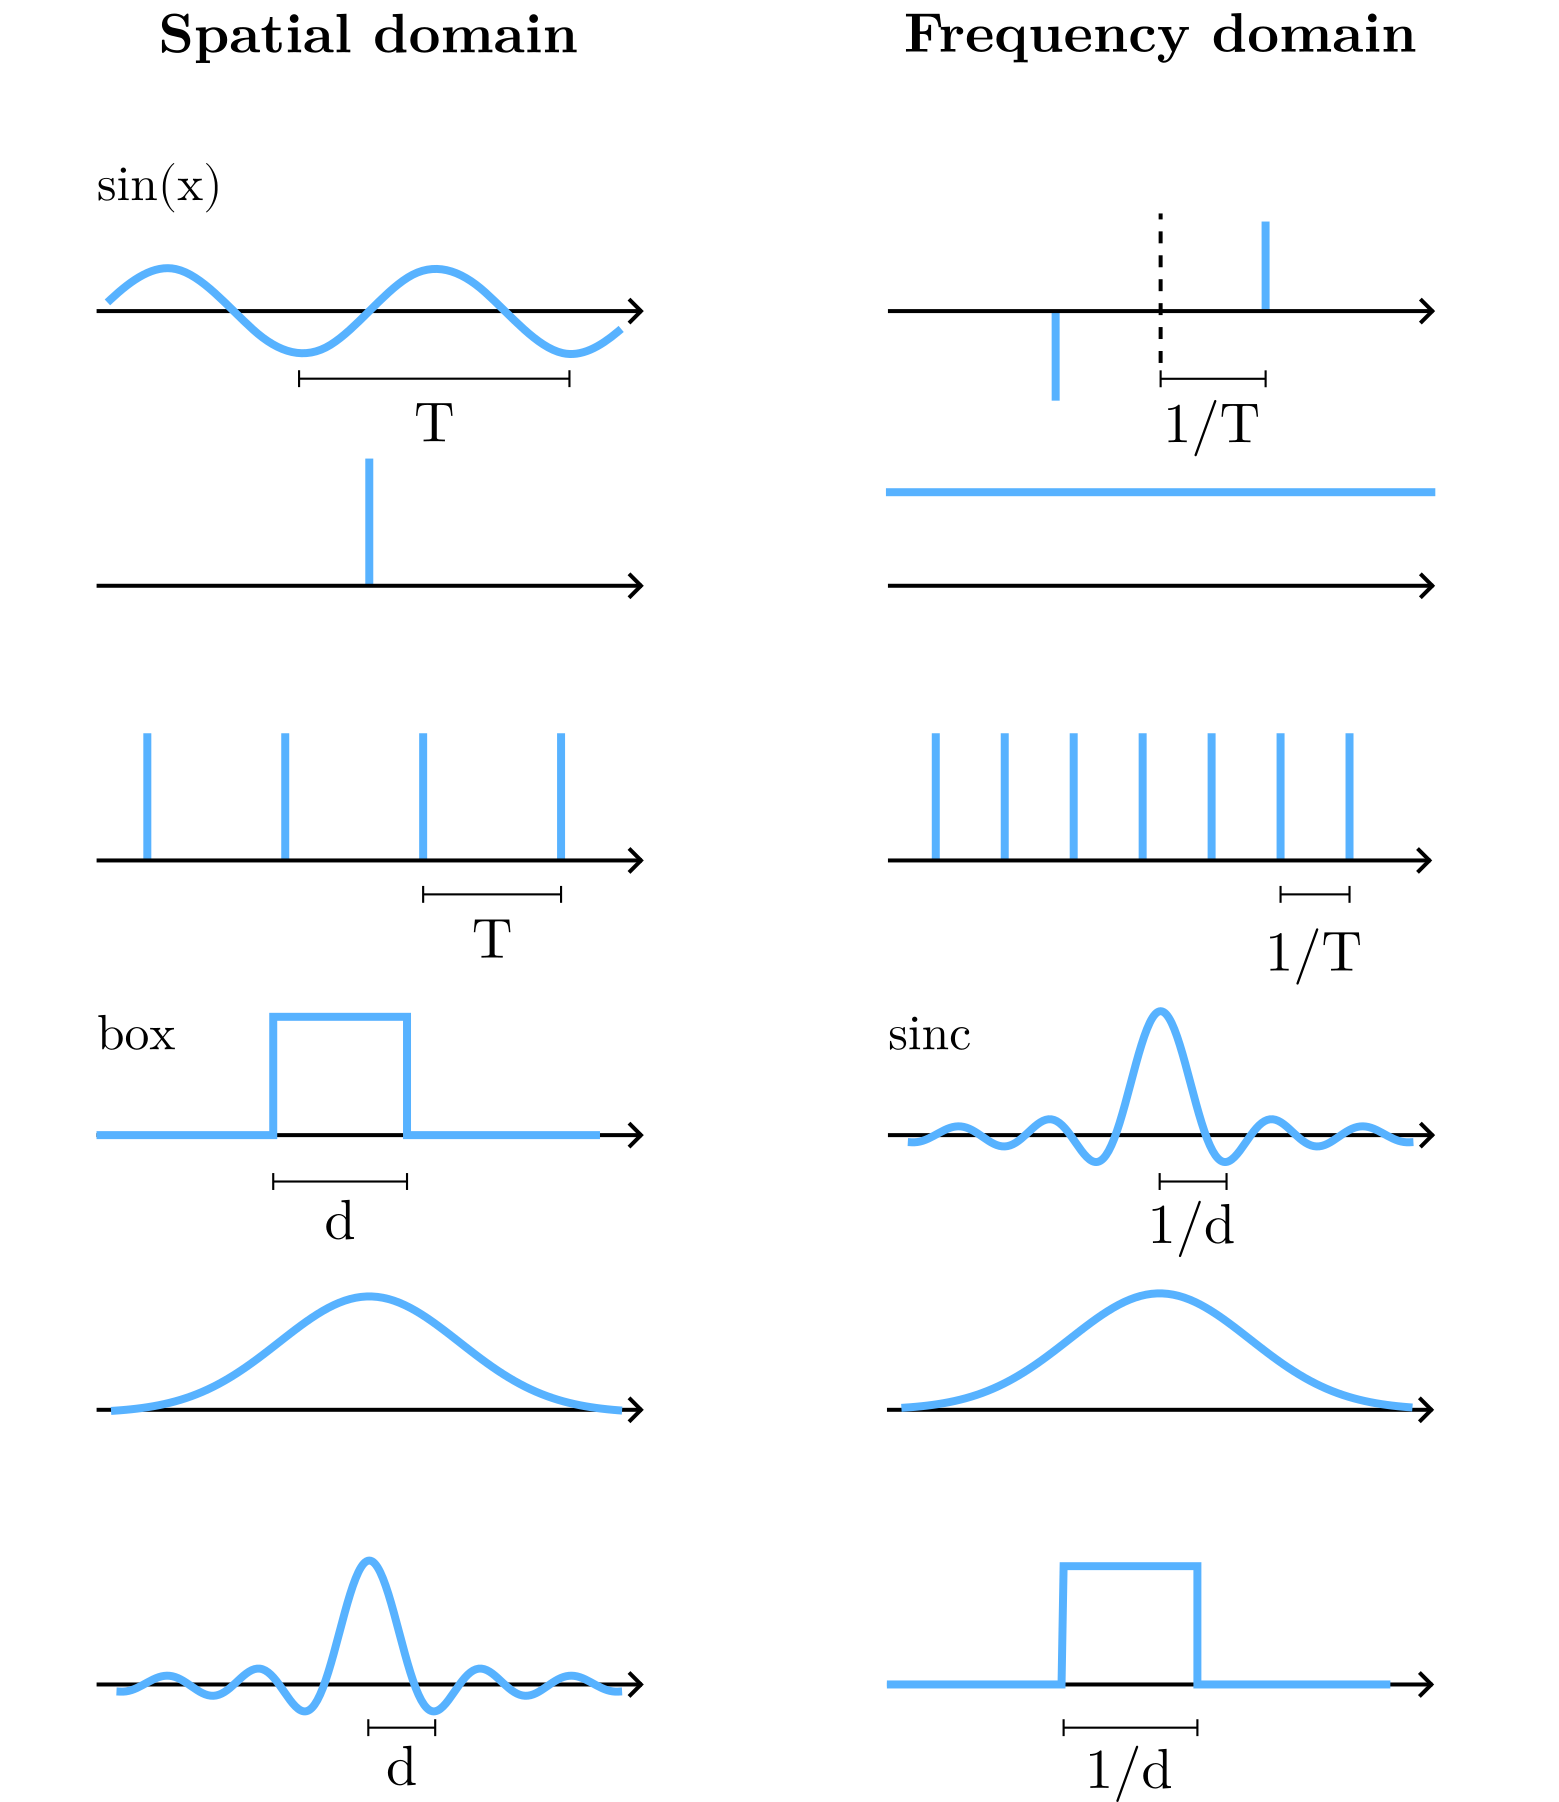
\includegraphics[width=\linewidth]{fourier-transforms.png}
\end{center}
% TODO: Rest of the FFT part

\subsection{PCA (also: KL transform)}
Given data \( x \in A \), e.g. an image, we want to compress it to a lower-dimensional space \( B \) with a compressor \( f: A \to B \) s.t. \( \text{size}(f(x)) \ll \text{size}(x) \). Minimize reconstruction error \( E = \Vert x - f^{-1}(f(x)) \Vert \) and maximize the variance of our encoding. Given \( N \) data samples \( x_i \in \mathbb{R}^d \):
\begin{enumerate}
    \item Normalize to remove brightness variations: \( x'_i = \sfrac{x_i}{\Vert x_i\Vert} \)
    \item Center data by subtracting mean: \( x''_i = x'_i - \mu, \quad \mu = \frac{1}{N}\sum x'_i  \)
    \item Compute covariance matrix: \( \Sigma = \frac{1}{N-1}\cdot \sum (x''_i)\cdot (x''_i)^\top \)
    \item Compute eigendecomp. of \( \Sigma \) by solving \( \Sigma e = \lambda e \) with e.g. SVG, i.e. \( \Sigma = U \Lambda U^\top \)
    \item Define \( U_k \) as the first \( k \) eigenvalues of \( \Sigma = \left[u_{1}, \ldots, u_k\right] \), dirs with largest variance (= eigenvalues)
    \item \( \text{PCA}(x_i) = U^\top_k (x_i - \mu) = U^\top_k \cdot x''_i \)
\end{enumerate}
To decompress, use \( \text{PCA}^{-1}(y_i) = U_k\cdot y_i + \mu  \).
\begin{itemize}
    \item Face recognition, compare in projected space and find nearest neighbour
    \item Face location, compute reconstruction error for every small patch, pick min
    \item Data compression and visualization
\end{itemize}
Eigenfaces struggle with different lighting conditions. Fisherfaces perform better by trying to maximize between-class scatter and minimizing within-class scatter.

\subsection{JPG}
\begin{enumerate}
    \item Conversion RGB \( \to \) YUV; only Y carries brightness info (luminance), UV contain color (chrominance)
    \item Humans are more sensitive to brightness than color, so compress colors with chroma subsampling (e.g. only color of upper left pixel for \( 4\times 4\) grid).
    \item Go over image with \( 8 \times 8 \) block for each YUV component and apply 2D DCT to it \( \rightarrow 64 \) vals, top left low.freq, bottom right high-freq.
    \item Compress by integer division with weighting matrix \( \rightarrow \) compress low-right
    \item Zig-zag run length encoding followed by Huffman
\end{enumerate}
High compression (10-100x) and 24 bit color depth is possible, but at the same time artifacts / wrong colors / Moiré. Also edges are softened because sharp edges require \( \infty \) freq.\\
JPEG2000 achieves better results by using the Haar transform globally, not just \( 8 \times 8 \), on a successively downsampled image.

\subsection{Optical Flow}
\textbf{Brightness Constancy}
\begin{align*}
    I(x,y,t) &= I(x+ \delta x, y + \delta y, t + \delta t) \\
	     &\approx I(x,y,t) + I_x \delta x + I_y \delta y + I_t \delta t \\
    \implies &I_x \delta x + I_y \delta y + I_t \delta t \approx 0 \\
    \implies &I_x \underbrace{\frac{\delta x}{\delta t}}_u + I_y \underbrace{\frac{\delta y}{\delta t}}_v I_t \approx 0
\end{align*}
\subsubsection{Aperture problem} 2 unknowns for every pixel \( (u,v) \) but only one equation \( \implies \infty\)  solutions, opt. flow constraint defines a line in \( (u,v) \) space, can compute normal flow. We therefore need an additional constraint for computation
\subsubsection{Horn \& Schunck} Assumption: values \( u(x,y), v(x,y) \) are smooth and change slowly with \( x,y \implies \) Minimize \( E = E_s + \lambda E_c, \lambda > 0 \) where 
    \begin{flalign*}
	E_c &= \iint (I_x u + I_y v + I_t)^2 \mathop{dx} \mathop{dy} && \text{(brightness constancy)} \\ 
	E_s &= \iint (u^2_x u^2_y) + (v^2_x + v^2_y) \mathop{dx} \mathop{dy} && \text{(smoothness)}
    \end{flalign*}
Has errors at boundaries / information spreads from corner-type patterns
\subsubsection{Applications} Frame extrapolation, frame interpolation, video compression (exploit temp. red.), structure from motion, object tracking, video stabilization (aim at OF \( \approx 0 \))
\subsubsection{Lucas-Kanade} Assume all neighbouring pixels in a patch \( W \) observer the same motion \( \left[ u,v \right]^\top \) (+ small movement, brightness constancy). Minimize \[ E = \sum_{(x,y)\in W} (I_x(x,y)u + I_y(x,y)v + I_t(x,y))^2 \] Solve least squares:
    \[
	\left[
	\begin{smallmatrix} 
	    \sum_W I^2_x & \sum_W I_x I_y \\
	    \sum_W I_x I_y & \sum I^2_y \\
	\end{smallmatrix}
	\right]
	\left(
	    \begin{smallmatrix}
		u \\ v
	    \end{smallmatrix}
	\right)
	= -
	\left(
	\begin{smallmatrix}
	    \sum_W I_x I_t \\
	    \sum_W I_y I_t
	\end{smallmatrix}
	\right)
    \] 
Fails if all gradients are in the same direction, e.g. for edges or smooth regions. However, it works well for corners and textured areas.
\subsubsection{Iterative refinement} Obtain more exact estimate of optical flow:
    \begin{enumerate}
	\item Estimate OF with Lucas-Kanade
	\item Use estimated flow to warp image
	\item Estimate OF using warped image
	\item Repeat
	\item Add up all estimates
    \end{enumerate}
    Fails if intensity structure poor or large displacement.
\subsubsection{Coarse-to-fine pyramids} Create multiple levels by gradual subsampling of the image. Start with coarsest level, estimate OF. Gradually use aggregated OF estimate as initial estimate of the OF in the next finer level and estimate again with Lucas-Kanade. Iterate until finest level. This still fails if large lighting change happens.

\subsection{Video Compression}
\subsubsection{Bloch's law} If stimulus duration \( \le \qty{100}{\milli\second}\), we can exchange duration for brightness and vice-versa, e.g. if brightness of stimulus is halved, double the duration \( \rightarrow \) can still be detected. This enforces \( > \qty{10}{\hertz} \) for videos
\subsubsection{Temporal redundancy} - exploit temp. red. by predicting current frame based on previously coded frames. There are 3 types of frames:
    \begin{itemize}
	\item \textit{I-Frame} - intra-coded frame, coded indep. of others (use e.g. JPG for spatial red.)
	\item \textit{P-Frame} - predictively coded frame based on prev. coded I- and P-frames
	\item \textit{B-Frame} - bi-directionally predicted frame, coded based on both prev. and future frames
    \end{itemize}
    This is ineffective if there are many scene changes and/or high motion

\begin{wrapfigure}{r}{1.5cm} 
    \centering 
    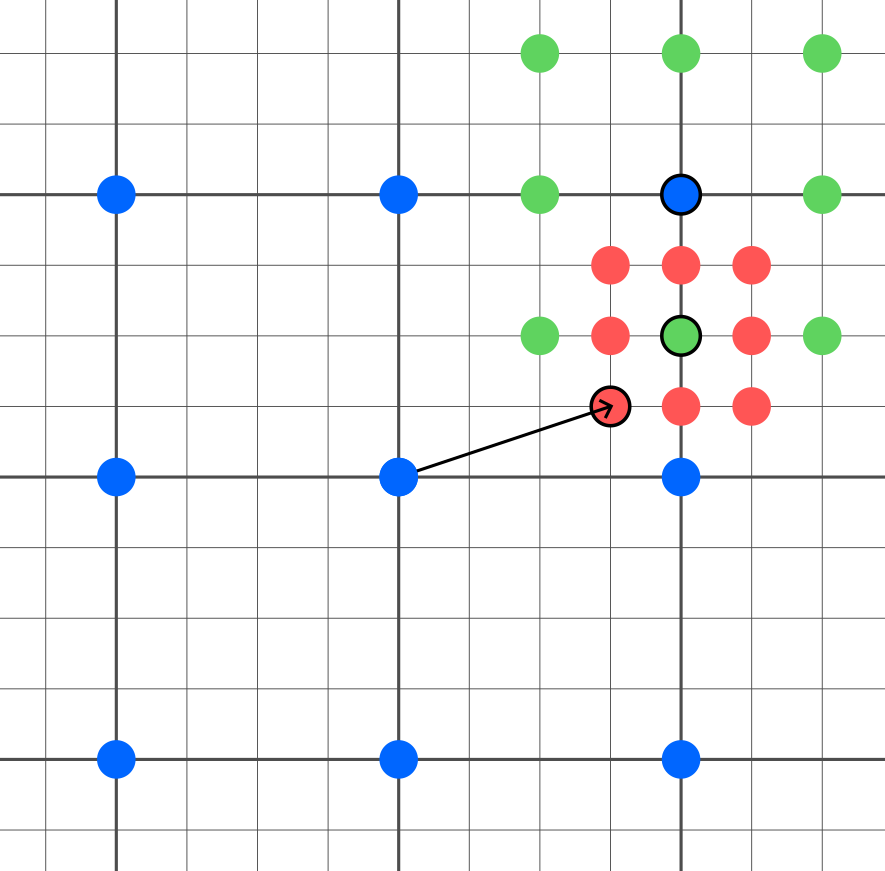
\includegraphics[width=1.5cm]{three-step-search.png}
\end{wrapfigure}

\subsubsection{Motion-compensated prediction} - use if temp. red. fails. Generally very difficult, pratical: \textit{block-matching motion estimation}. Partition each frame into blocks and describe motion by finding best matching block in reference frame

\begin{itemize}
    \item can be sped up with 3-step search
    \item can increase precision by using half-pixel motions (interpolation needed)
\end{itemize}
After performing motion prediction, we encode the error between the actual frame and the motion constructed one (e.g. with JPG).
This assumes a translation model which brekas down for complex motion and produces blocking artifacts. However, the performance is good, the structure is simple and periodic, the motion vector field is easy to represent and half-pixels reduce noise \& prediction error, thus better compression.
\subsubsection{MPEG Group of Pictures (GOP)} - starts with I-frame, ends with B-frame (``open'') or P-frame (``closed'')

\subsection{Conv. Neural Networks}
Given a kernel with size \( F \), an image with size \( N \), padding \( P \) and a stride \( S \), the output dimensions of applying the filter to the image is \( \frac{N+2P-F}{S} + 1 \). For stride \( 1 \) and padding \( P = \sfrac{F-1}{2} \), the input dimension is thus preserved.

\subsection{Radon Transform}
Given an object with unknown density \( f(x,y) \), find \( f \) by sending rays from all dirs through the object and measure absorption on the other side. We assume parallel beams for a given angle and no spreading of a beam.

Basic concept of image reconstruction:
% TODO
Continous case: The radon transform of a line is \( R(\rho , \theta) = \int u(\rho \cos (\theta ) - s \sin (\theta ), \rho \sin (\theta ) + s \cos (\theta )) \mathop{ds} = \iint_{\mathbb{R}^2} u(x,y) \delta (p - x \cos \theta - y \sin \theta ) \mathop{dx} \mathop{dy} \). We want to find the optical density \( u(x,y) \) given \( R(\rho , \theta ) \).

\begin{itemize}
    \item Linear
    \item Input shifted \( \implies \) RT shifted
    \item Coordinate system rotated \( \implies \) RT rotated
    \item RT of 2D convolution is a 1D conv. of RT'ed functions with respect to \( \rho \) (\( R(f*_\text{2D} g) = R(f) *_\text{1D} R(g) \), rhs. with fixed \( \theta  \))
\end{itemize}
\textbf{Back projection} - given RT, find \( u(x,y) \). Example: \\ %TODO 
\textbf{Fourier / Central Slice Theorem} - % TODO

\section{Computer Graphics}
\subsection{Graphics Pipeline}
\begin{enumerate}
    \item Modeling Transform - from oject to world space
    \item Viewing Transform - from world to camera space, want z-axis = dist. to object
    \item Primitive Processing - output primitives from transformed vertices
    \item 3D Clipping - remove unneeded primitives with view frustum, occlusion and back face culling
    \item Projection to Screen Space
    \item Scan Conversion - discretize continous primities, interpolate attributes from vertices to pixel granularities (e.g. normals, UV)
    \item Lighting, Shading, Texturing - compute color based on lighting shading and texture map
    \item Occlusion Handling - handle occlusions, e.g. with z-Buffer
    \item Display result
\end{enumerate}

\subsubsection{Fragment} Generalization of a pixel that stores info such as depth or texture coords in addition to color

\subsection{Light \& Colors}

\subsection{Transformations}
\subsubsection{Homogeneous coordinates}
Allow representing translation by matrix multiplication, done by projection onto hyperplane: \( p = \left[\begin{smallmatrix}x & y & z & w\end{smallmatrix}\right]^\top \to \left[\begin{smallmatrix}\frac{x}{w} & \frac{y}{w} & \frac{z}{w} & 1\end{smallmatrix}\right] \)

\subsubsection{3D Transformations} Examples: \\ 
\bgroup
\setlength{\tabcolsep}{0.2em}
\begin{tabularx}{\linewidth}{lllX}
    Trans. & \( \left[\begin{smallmatrix} 1 & 0 & 0 & t_x \\ 0 & 1 & 0 & t_y \\ 0 & 0 & 1 & t_z \\ 0 & 0 & 0 & 1 \end{smallmatrix}\right]  \) & 
    Scaling & \( \left[\begin{smallmatrix} s_x & 0 & 0 & 0 \\ 0 & s_y & 0 & 0 \\ 0 & 0 & s_z & 0 \\ 0 & 0 & 0 & 1 \end{smallmatrix}\right]  \) \\
    Rot. (x) & \( \left[\begin{smallmatrix} 1 & 0 & 0 & 0 \\ 0 & \cos \theta & -\sin \theta & 0 \\ 0 & \sin \theta  & \cos \theta & 0 \\ 0 & 0 & 0 & 1 \end{smallmatrix}\right]  \) &
    Rot. (y) & \( \left[\begin{smallmatrix} \cos \theta  & 0 & \sin \theta  & 0 \\ 0 & 0 & 1 & 0 \\ -\sin \theta & 0 & \cos \theta & 0 \\ 0 & 0 & 0 & 1 \end{smallmatrix}\right]  \) \\
    Rot. (z) & \( \left[\begin{smallmatrix} \cos \theta  & -\sin \theta & 0 & 0 \\ \sin \theta & \cos \theta & 0 & 0 \\ 0 & 0 & 1 & 0 \\ 0 & 0 & 0 & 1 \end{smallmatrix}\right]  \) &
    Shear (2D) & \( \left[\begin{smallmatrix} 1 & a & 0 \\ 0 & 1 & 0 \\ 0 & 0 & 1 \end{smallmatrix}\right]  \) \\
    Shear (x) & \( \left[\begin{smallmatrix} 1 & 0 & \text{sh}_x & 0 \\ 0 & 1 & \text{sh}_y & 0 \\ 0 & 0 & 1 & 0 \\ 0 & 0 & 0 & 1 \end{smallmatrix}\right]  \) & \\
\end{tabularx}
\egroup

\subsubsection{Commutativity}
\( M_1 M_{2} = M_{2} M_{1} \) holds for
\begin{center}
    {\renewcommand{\arraystretch}{1.2}
    \begin{tabularx}{\linewidth}{c>{\centering\arraybackslash}Xc>{\centering\arraybackslash}Xc}
	\toprule
	\( M_{1} \) & \( M_{2} \) & \\
	\midrule
	Translation & Translation & \\
	Rotation & Rotation & (only in 2D!) \\
	Scaling & Scaling &\\
	Scaling & Rotation & \\
	\bottomrule
    \end{tabularx}
    }
\end{center}

\subsubsection{Change of coord. system} Visually:

\begin{figure}[h]
    \center
    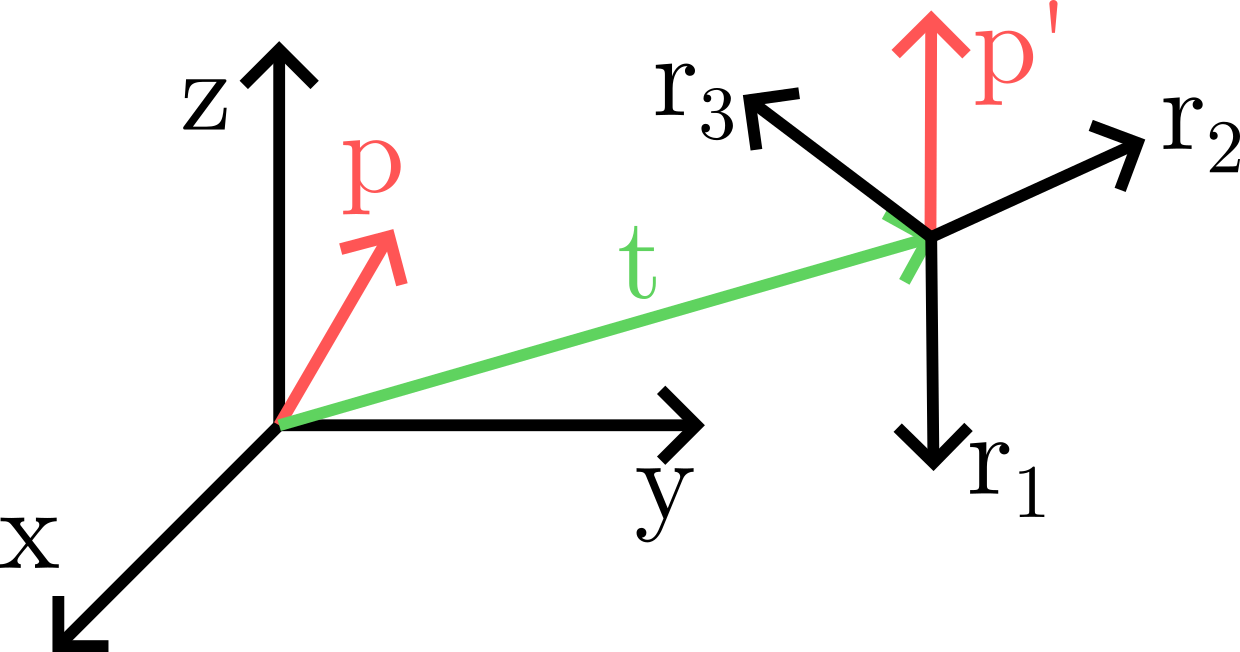
\includegraphics[width=2.5cm]{coord-system-change.png}
\end{figure}
\[ p' = \left[\begin{smallmatrix} | & | & | & | \\ r_1 & r_2 & r_2 & t \\ | & | & | & | \\ 0 & 0 & 0 & 1 \end{smallmatrix}\right] \implies p' = TRp \]
Transforming a normal \( n \): \( n' = (M^{-1})^\top n \)

\subsubsection{Quaternions} Alternative approach for rotation. \\
Properties:
\begin{align*}
	i^2=j^2=k^2 = -1, \quad ijk = -1, \quad ij=k, \quad ji=-k \\ \quad jk=i, \quad kj = -i, \quad ki = j, \quad ik = -j \\
	\lVert q \rVert = \sqrt{a^2+b^2+c^2+d^2},\\ \text{where } q = a + \left[\begin{smallmatrix} b & c & d \end{smallmatrix}\right] \left[\begin{smallmatrix} i \\ j \\ k \end{smallmatrix}\right] = a + v \text{ ,v not vector!} \\
	\overline{z} = a - bi - cj - dk, \quad z^{-1} = \frac{\overline{z}}{\lVert z \rVert}
\end{align*}

\subsubsection{Rotation with quaternions} Rotate \( p = \left[\begin{smallmatrix} x & y & z \end{smallmatrix}\right] \) around axis \( u = \left[\begin{smallmatrix} u_{1} & u_{2} & u_{3} \end{smallmatrix}\right] \) by angle \( \theta  \).
\begin{enumerate}
    \item Convert \( p \) to quaternion \( p_Q = xi + yj + zk \)
    \item Convert u to quaternion \( q'' = u_{1}i+u_{2}j+u_{3}k \) and \\ normalize \( q'' \) to \( q' = \sfrac{q''}{\lVert q'' \rVert} \)
    \item Rotation quaternion \( q = \cos (\theta /2) + \sin (\theta /2) q' \) \\ and \( q^{-1} = \cos (\theta /2) - \sin (\theta /2) q' \)
    \item Rotated point \( p' = q p q^{-1} \)
    \item Convert \( p' \) back to cartesian
\end{enumerate}

\subsubsection{Orientation of coord. system}
Thumb: x-axis, index finger: y-axis, middle finger: z-axis. To get direction of cross product, use thumb \& index finger as multiplicands and middle finger is direction.

\subsection{Lighting}
\subsubsection{Luminous Flux} \( \int P(\lambda)V(\lambda) \mathop{d\lambda} \) \\
Perceived power of light, weighted with human sensitivity [lumen] 
\subsubsection{Irradiance / Illumination} \( E(x) = \sfrac{d \phi(A)}{dA(x)} \) \\
Flux per unit area arriving at surface [\( \unit{W /m^2} \)]
\subsubsection{Radiosity} \( B(x) = \sfrac{d \phi (A)}{dA(x)} \; \left[\unit{W/m^2}\right] \) \\
Flux per unit area leaving a surface [\( \unit{W/m^2} \)]
\subsubsection{Radient/Luminous Intensity} \( I(\vec{w}) = \sfrac{d \phi}{d \vec{w}} \; \left[\unit{W/sr}\right] \) \\
Outgoing flux per solid angle [\( \unit{W/sr} \)]
\subsubsection{Radiance/Luminance} \( L(x, \vec{w}) = \sfrac{d^2 \phi (A)}{\cos \theta d A(x) d \vec{w}} \) \\
Flux per solid angle per perpendicular area = effective intensity per unit area
% TODO decipher georgette stuff

\subsubsection{Lighting} Modeling physical interactions between materials and light sources
\subsubsection{Shading} Process of determining the color of a pixel
\subsubsection{Phong Reflection / Illumination Model} 
\[
    I = \underbrace{I_a k_a}_{\text{ambient}} + f_{att} I_p [\underbrace{k_d(N\cdot L)}_{\text{diffuse}} + \underbrace{k_s(R\cdot V)^n}_{\text{specular}}]
\] 
\( R = N \cdot \cos (\theta) + S = 2N(N\cdot L) - L \).
Material parameters: \( k_a, k_d, k_s, n \),
light parameters: \( I_a, I_p \),
geometry parameters: \( N, L, V \). Increasing \( n \) leads to smaller highlights in terms of surface area. 

\subsection{Shading Models}
\subsubsection{Flat shading} One color per primitive
\subsubsection{Gouraud shading}
\begin{enumerate}
    \item Calculate face normals
    \item Calculate vertex normals by averaging (weighted by angle)
    \item Evaluate illumination model per vertex
    \item Interpolate vertex colors bilinearly on current scan line
\end{enumerate}
Problems with scan line interpolations are perspective distortion, orientation dependence and shared vertices. Quality depends on primitive size

\subsubsection{Phong shading} Barycentric interpolation of normals\\
\begin{figure}[h]
    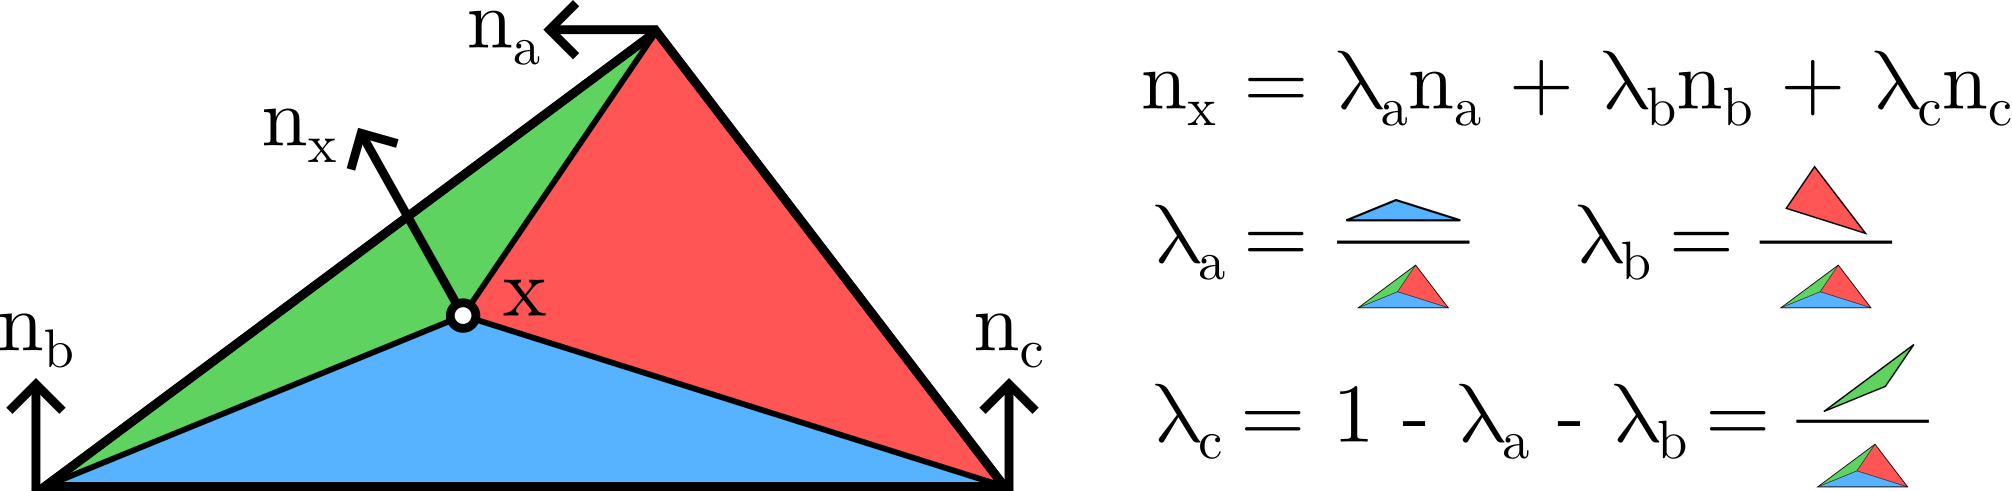
\includegraphics[width=\linewidth]{phong-shading.png}
\end{figure}

\noindent Properties: \( x = a \implies n_x = n_a, \quad \lambda_a+\lambda_b +\lambda_c = 1, \\ \lambda_a a+ \lambda_b b + \lambda_c c = x \)
Problem: The normal may not be defined or not representative.

\subsubsection{Transparency} \( I_\lambda = I_{\lambda_1} \alpha_1 \delta t + I_{\lambda_2} e^{-\alpha_1 \delta t} \implies \) linearization \( \implies I_\lambda = I_{\lambda_1} \alpha \delta t + I_{\lambda_2} (1-\alpha_1 \delta t) \). If it's the last object, set \( \delta t = 1 \). \\
Problem: Rendering order, we need sorted traversal of polygons \( \to  \) back-to-front rendering

% TODO: Transparency diagram

\subsection{Geometry \& Textures}
\subsubsection{Parametric Surface} \( (x(u,v), y(u,v), z(u,v)) \)
\subsubsection{Subdivision Surface} Define surface by primitives, use recursive algorithm for refining
\subsubsection{Implicit Surface} Zero set of a function
\subsubsection{Polygonal Mesh} Explicit set of vertices with position + connectedness information. Every vertex can have additional attributes (color, normal)
\subsubsection{Texture Mappings} Goal: Map Texture \( (u,v) \)-coords. to geometry \( (x,y,z) \)-coords. Example of sphere mapping: \\\( (u,v) \to (\sin (u) \sin (v), \cos (v), \cos (u) \sin (v)) \). We want low distortion, a bijective mapping that is efficiently computable.
\subsubsection{Light Maps} Save computation power by precomputing static lighting and applying it to texture (can be dynamically adapted)
\subsubsection{Environment Maps} Mirror environment with imaginary sphere / cube for easier computation of reflective objects
\subsubsection{Bump Maps} Perturb normals to fake fine detail, store normal displacement in grayscale value. A \textbf{Normal map} directly stores perturbed normals as \( (r,g,b) \) color where \( n' = (2r - 1, 2g - 1, 2b -1)^\top \). Limitations: No bumps on silhouette, no self-occlusions, no self-shadowing. In contrast, \textbf{displacement mapping} actually modifies geometry, but more complex \& expensive
\subsubsection{Procedural Textures} Generate textures from noise, e.g. Perlin or Gabor noise by creating a gaussian pyramid of noise and summing all layers in a weighted way
\subsubsection{Mip-Mapping} Store down-sampled (blurred to avoid aliasing) versions of texture, use low-res versions for far away objects and interpolate inbetween. This avoids asliasing and improves compute efficiency but incurs a storage overhead
\subsubsection{Perspective Projection} Linear variations in world coordinates can yield non-linear variation in screen coords \( \to  \) optimal resampling filter is spatially variant
\subsubsection{Geometry aliasing} Happens at polygon edges. Solution: Introduce multiple samples per pixel (supersmapling). Different patterns possible: Uniform, jittering, stochastic, poisson, ...
%TODO small illustration

\subsection{Curves \& Splines}
\subsubsection{Bézier curves}
\( x(t) = b_0 B^n_0(t) + \ldots + b_n B^n_n (t) \) \\
\( B^n_i(t) = \binom{n}{i} t^i (1-t)^{n-i}, \text{ if } i < 0 \lor i >0 \implies B^n_i (t) = 0 \) \\
(reminder: \( \binom{n}{i} = \sfrac{n!}{i!(n-i)!} \)) The \( B^n_i \)'s are the Bernstein polynomials.
It can be constructed visually with the deCasteljau algorithm. 
% TODO illustration
\begin{citemize}
    \good arbitrary \# of control points
    \bad global support of basis func.
    \bad insertion of control point \( \to  \) higher degree
    \bad high degree results in oscillations
\end{citemize}

\subsubsection{B-splines}
\( x(t) = \sum_{i=0}^k d_i N_i^n (t) \), basis function is recursively defined by convolution of box func.: 
\( B^0(t) = 1 \text{ if } t \in [-1, 0] \implies B^1(t) = \int_\mathbb{R} B^0(s) B^0(t-s) \mathop{ds} \text{ und } B^n(t) = B^{n-1}(t) * B^0(t)\)

% TODO check which splies we had

\subsubsection{Subdivision Surfaces} Generalization of spline curves/ surfaces, converge to smooth limit surface, successive refinement.
\textit{Primal}: Faces are split into sub-faces,
\textit{Dual}: Vertices are split into multiple vertices
\textit{Approx.}: Control points are not interpolated
\textit{Interpol.}: Control points are interpolated

\begin{center}
    \renewcommand{\arraystretch}{1.2}
\begin{tabularx}{\linewidth}{Xccc}
    \toprule
    & \multicolumn{2}{c}{\textbf{Primal}} & \textbf{Dual} \\
    & Triangles & Rectangles & \\
    \midrule
    \textbf{Approx.} & Loop & Catmull-Clark & Doo-Sabin \\
    \textbf{Interpol.} & Butterfly & Kobbelt & \\
    \bottomrule
\end{tabularx}
\end{center}

\subsection{Scan Conversion}
\subsubsection{Bresenham line} Always choose closest pixel at each intersection. 
% TODO illustration
After having computed the first \( d \) we can get the following \( d_\text{new} \) by adding \( a \) if we chose east (so \( d < 0 \)) or adding \( a + b \) if we chose north-east \( d > 0 \), which makes it very fast.

\subsubsection{Scan Conversion of Polygons} 
\begin{enumerate}
    \item Calculate all intersections on scan line
    \item Sort intersection points by ascending x-coordinates
    \item Fill all spans between consecutive intersections if parity is odd
\end{enumerate}
% TODO: small illustration

\subsection{Visibility \& Shadows}
\subsubsection{Painter's Algorithm} Solves visibility problem by rendering objects from furthest to nearest. Has issues with cyclic overlaps \& intersections
\subsubsection{Z-buffering} Store depth of nearest object for each pixel. Initialize all values to \( \infty \), then iterate over polygons and update z-buffer.
Limited resolution can cause flickering, so place near clipping plane far from camera.

\subsubsection{Planar Shadows} Draw projection of object onto ground. No self-shadows, no shadows on other object, curved surfaces
\subsubsection{Projective Texture Shadows} Separate obstacles and receivers, generate b/w image of the obstacle from light \( \to  \) use img as proj. texture. Need to specify obstacles \& receivers, no self-shadows
\subsubsection{Shadow Maps} Compute depths from light, compute depths from camera. For each pixel on camera plane, compute point in world coords., then project point onto light plane and compare \( a \) and \( b \), \( a + \text{bias} < b \implies \) in shadow. Bias needed to avoid self-shadowing, point can lie outside FoV of shadow map (\( \to \) use cubical shadow map) and aliasing due to undersampled shadow map (\( \to  \) filter result of depth test, not depths)
%TODO: small illustration

\subsubsection{Shadow Volumnes} Explicitly represent shape of space in shadow as volume. Shoot ray from camera, incr./decr. each time a volume is entered/left \( \implies > 0 \implies \) in shadow. (Optimization: Use silhouette edges only.) Introduces lots of new geometry, expensive, objects must be watertight for silhouette optimization

\subsection{Ray Tracing}
For each pixel, send a ray into the scene. On object hit, send multiple rays (diff., reflected, refracted) further until we hit a light source or reach some \# of bounces. Figure out whether point in shadow by shooting rays to all light sources. For anti-aliasing, use multiple rays per pixel.

\subsubsection{Ray-Surface Intersections} Ray equation: \( r(t) = o + td \)
Sphere intersection: Solve for \( t: \lVert o + td - c \rVert ^2 - r^2 = 0 \) \\
Triangle: first intersect with triangles plane: \( t = -\frac{(o+p_{1})n}{dn} \), where \( n = (p_{2}-p_{1})\times(p_{3}-p_{1}) \).
Then compute barycentric coeff. of intersection point and check whether \( s_{1}+s_{2}+s_{3} = 1 \land 0 \le s_i \le 1 \implies \) if yes, inside triangle

\subsubsection{Ray Tracing Extensions}
\begin{itemize}
    \item Add refraction
    \item Add area lights by having multiple shadow rays
    \item Motion blur: render objects at diff. times per frame
    \item Depth of field
\end{itemize}

\subsubsection{Acceleration Data Structures}
\smallskip
\subsubsection{Brute force} Intersect every ray with every primitive
\subsubsection{Uniform grids} Determine grid resolution, compute AABB's, incrementally rasterize ray, compute intersection with objects in each cell, stop when intersection found, if multiple take closest.
\begin{citemize}
    \good easy to code
    \good building data structure is fast
    \bad does not adapt to non-uniform scenes (\( \to  \) hierarchical grids)
\end{citemize}
\subsubsection{Space partitioning trees} Octree, kd-tree, bsp-tree

\end{document}
